\newpage % Rozdziały zaczynamy od nowej strony.
\cleardoublepage % Zaczynamy od nieparzystej strony
\pagestyle{headings}
\section{Wstęp}

\subsection{Wprowadzenie}

W ostatnich latach można zaobserwować gwałtowny rozwój w dziedzinie 
Uczenia Maszynowego (ang. \emph{Machine Learning}) i Sztucznej Inteligencji 
(ang. \emph{Artificial Intelligence}). Coraz więcej urządzeń staje się systemami działającymi autonomicznie, bez potrzeby ingerencji człowieka. 
Jednym z algorytmów, który powstał już dość dawno, są Sztuczne Sieci Neuronowe (ang. \emph{Artificial Neural Networks}). Temat Sieci Neuronowych ma długą historię rozwoju, sięgającą początku lat 40. XX wieku, jednak w ostatnich latach można zaobserwować znaczny postęp w tej dziedzinie \cite{Kriesel2007NeuralNetworks}. Rozwój technologii umożliwił zastosowanie algorytmów AI w wielu aplikacjach. Działalność naukowa w kierunku Sztucznych Sieci Neuronowych spowodowała powstanie nowych modeli i architektur.

Większość algorytmów wykorzystujących Sztuczną Inteligencję wymaga dużej mocy 
obliczeniowej i wyboru odpowiedniego sprzętu. Często powtarzaną operacją matematyczną 
w przypadku algorytmu Sztucznej Sieci Neuronowej jest mnożenie macierzy.
Działanie to można w łatwy sposób zrównoleglić, implementując sieć w układzie 
FPGA i tym samym zwiększyć efektywność algorytmu.

Praca nad implementacją algorytmów Sztucznej Inteligencji w większości 
przypadków zaczyna się od stworzenia i uruchomienia modelu. Do tego zadania 
często wykorzystywane są wysokopoziomowe biblioteki takie jak \emph{Keras} lub \emph{Theano}, które w znacznym stopniu przyspieszają proces tworzenia oprogramowania oraz ułatwiają wprowadzanie zmian w modelu sieci. Rozwój i dopracowywanie 
algorytmu Sztucznej Inteligencji wymaga wielu iteracji uruchamiania kodu 
z różnymi parametrami i właściwościami sieci. Aby w pełni wykorzystać potencjał Sztucznych Sieci Neuronowych, należy dobrać odpowiednią metody projektowania i testowania modeli.

\subsection{Wstęp teoretyczny}

Sieć neuronowa jest algorytmem przetwarzającym dane, inspirowanym działaniem mózgu.
ANN składa się z wielu elementów przetwarzających informacje -- neuronów. Model
przetwarzania informacji jest inspirowany ludzkim mózgiem jednak w stosunku do
komórki nerwowej, Neuron w Sztucznej Sieci Neuronowej jest bardzo uproszczony
\cite{tadeusiewicz1993sieci}. Pomimo to ANN umożliwiają rozwiązywanie złożonych
problemów w wielu dziedzinach z dużą dokładnością.

Neurony są połączone ze sobą krawędziami sieci. Każda krawędź ma swoją wagę, która 
zmienia wartość w trakcie uczenia sieci. Warstwę sieci, w której wszystkie wyjścia każdego z neuronów są podłączone do wszystkich neuronów w warstwie następnej, nazywa się warstwą w pełni połączoną (ang. FC — \emph{Fully Connected}).
Sieć posiadająca wszystkie warstwy w pełni połączone jest zwana siecią w pełni połączoną. 

W znacznej większości sieci neuronowe budowane są w ten sposób, że dane są propagowane w kierunku od warstwy wejściowej do wyjściowej. Takie sieci nazywamy sieciami jednokierunkowymi (ang. \emph{feedforward}). Przykładową sieć neuronową w pełni połączoną typu \emph{feedforward} przedstawiono na Rys. \ref{ann-img}.
\bigskip

\begin{figure}[h]
  \centering
  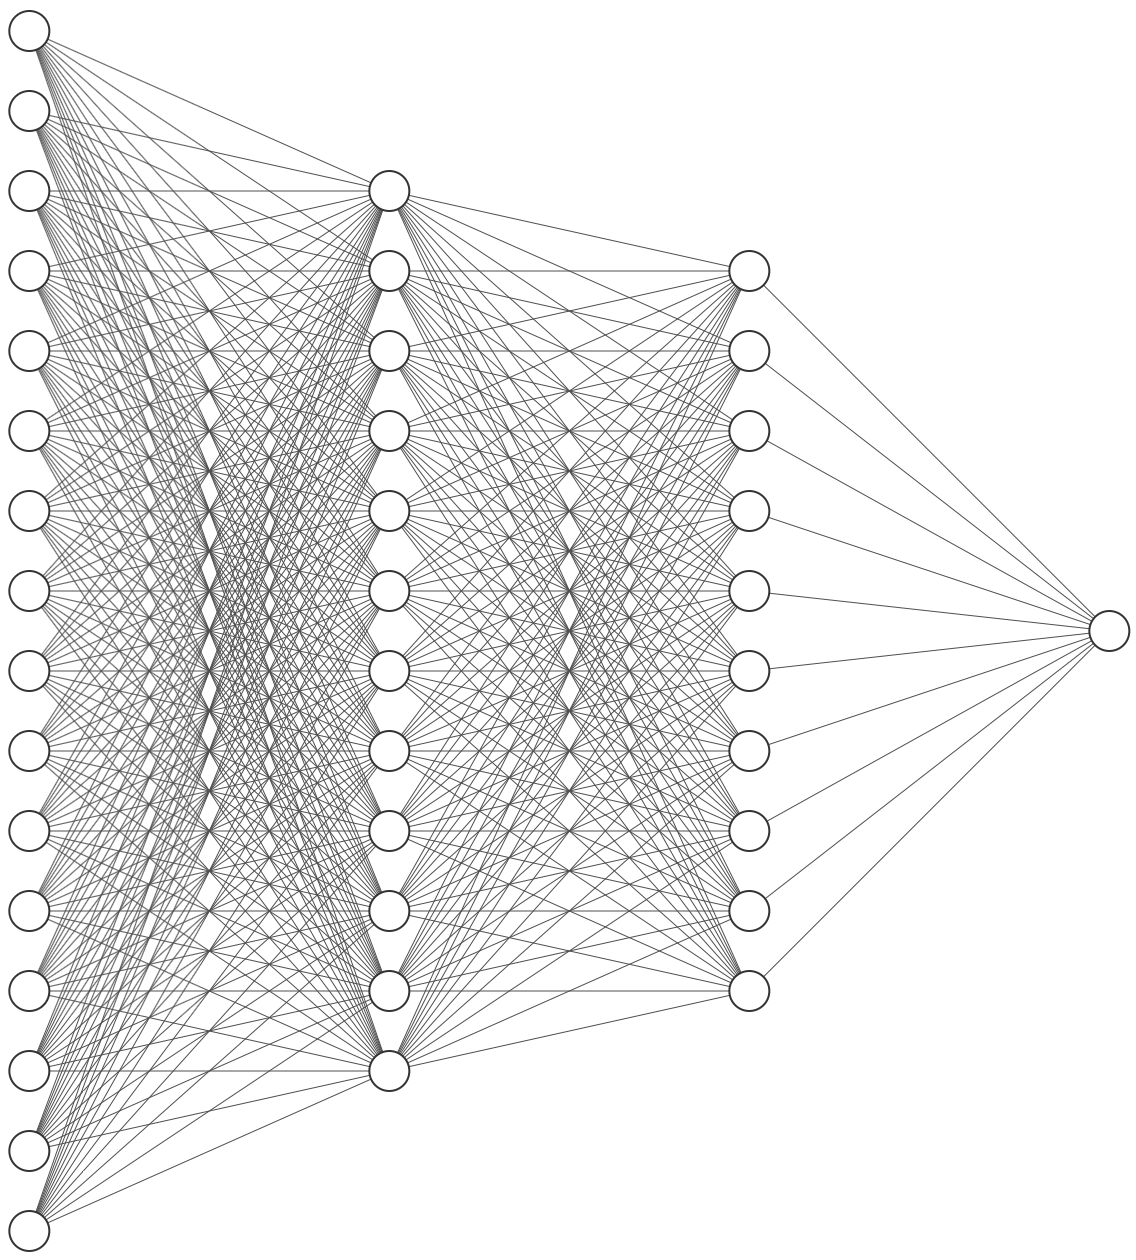
\includegraphics[width=0.8\textwidth]{img/ann.png}
  \caption{Schemat w pełni połączonej jednokierunkowej Sieci Neuronowej}
  \label{ann-img}
\end{figure}


\subsubsection{Model neuronu}
Sztuczne Sieci Neuronowe to algorytm wzorowany działaniem ludzkiego mózgu 
i znajdujących się w nim neuronów. Model matematyczny (Rys. \ref{neuron}) pojedynczego 
neuronu — Perceptron\cite{Omondi2006FPGAIO} składa się z następujących elementów:
\begin{itemize}
  \item wektora wejściowego: 
  $$x = (x_1, x_2,...,x_j)^T$$
  \item wektora wag przypisanych do każdego z wejść
  $$w = (w_{k1}, w_{k2},...,w_{kj})^T$$
  \item wag obciążających (bias) $b$
  \item funkcji aktywacji $\phi(u)$ 
  \item wyjścia neuronu $y$. 
\end{itemize}
Wagi obciążające (bias) umożliwiają, niezależnie od wartości wejściowych, kontrolowanie progu aktywacji neuronu. W praktyce oznacza to przesuwanie wykresu funkcji aktywacji w kierunku poziomym. Wyjście neuronu można policzyć stosując następujące wzory:
$$u_k = \sum_{j=1}^{N}{w_{kj}x_j} $$ 
$$y_k = \phi(u_k + b_k) $$ 


\begin{figure}[h]
  \centering
  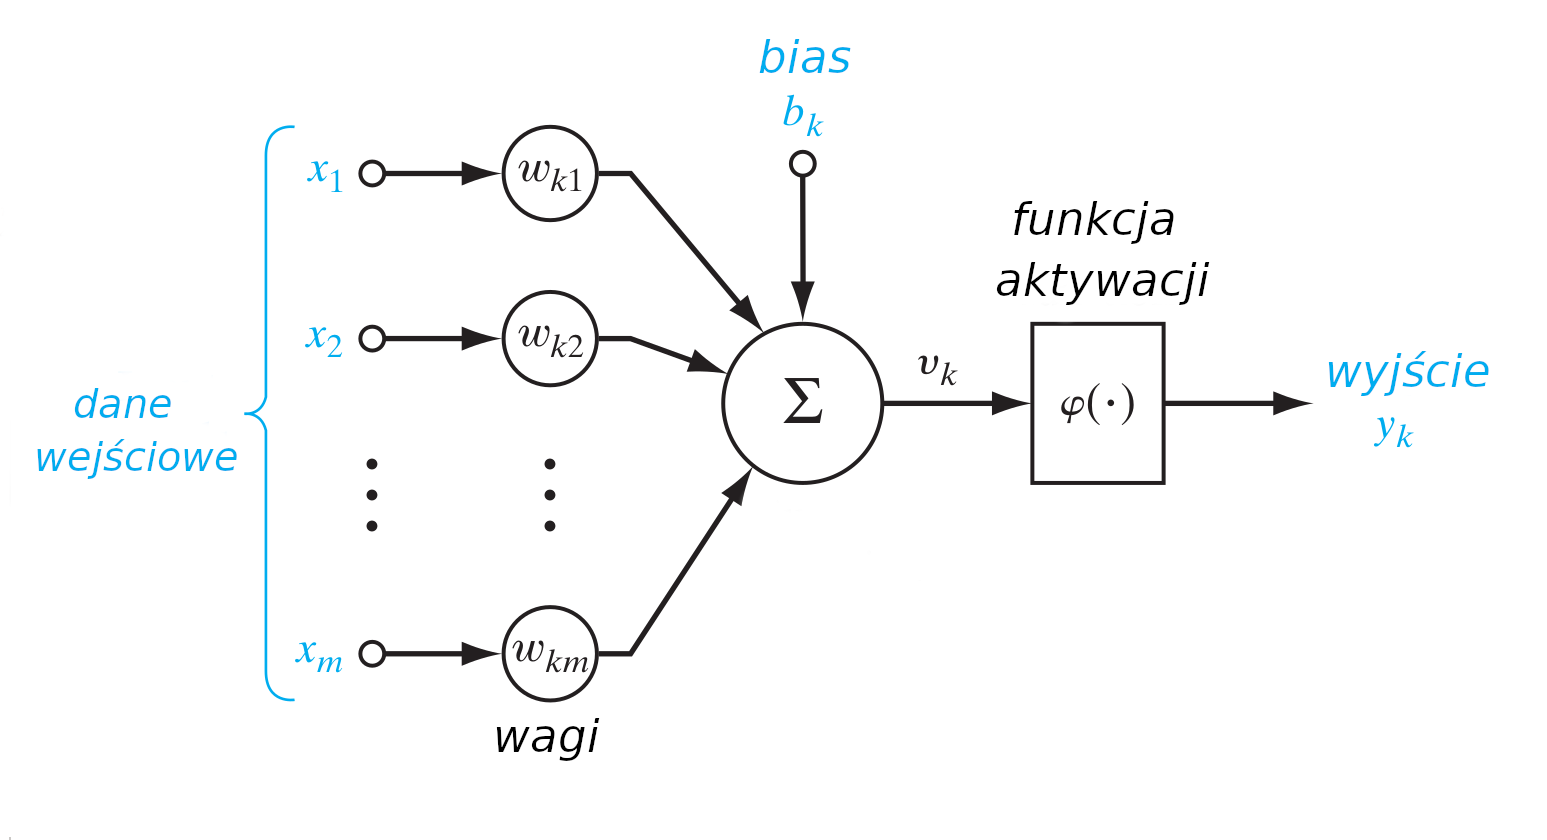
\includegraphics[width=\textwidth]{img/neuron.png}
  \caption{Model neuronu}
  \label{neuron}
\end{figure}


\subsubsection{Funkcja aktywacji}
Na działanie algorytmu znaczny wpływ może mieć dobór odpowiedniej 
funkcji aktywacji. Wśród najczęściej stosowanych funkcji aktywacji
wyróżnia się następujące funkcje:
\begin{itemize}
    \item funkcja ReLu (ang. \emph{Rectified Linear Units}): 
    
    $$\phi(x) = max(0, x)$$
    \begin{figure}[!h]
      \centering
      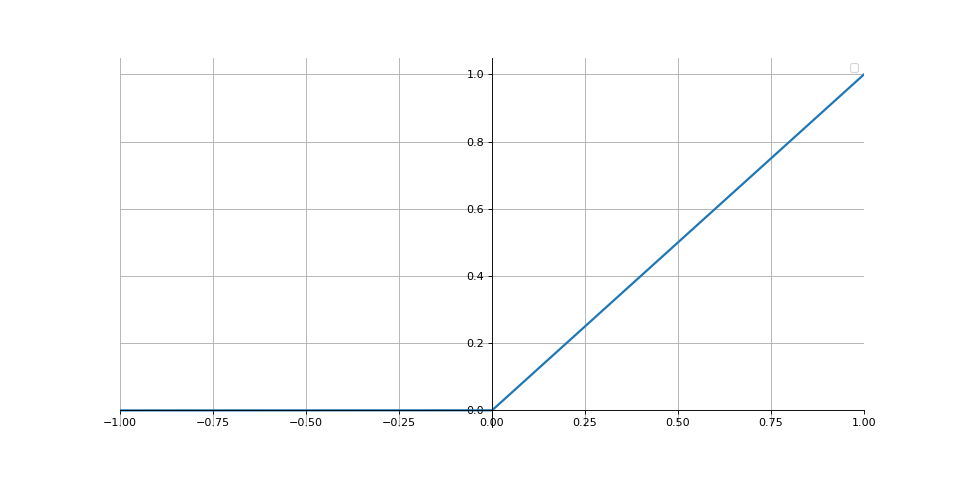
\includegraphics[width=\textwidth]{img/relu.png}
      \caption{Wykres funkcji ReLU}
      \label{sigmoid}
    \end{figure}

    \item funkcja sigmoid: 
    
    $$\phi(x) = \frac{a}{a + e^{-bx}}$$
    \begin{figure}[!h]
      \centering
      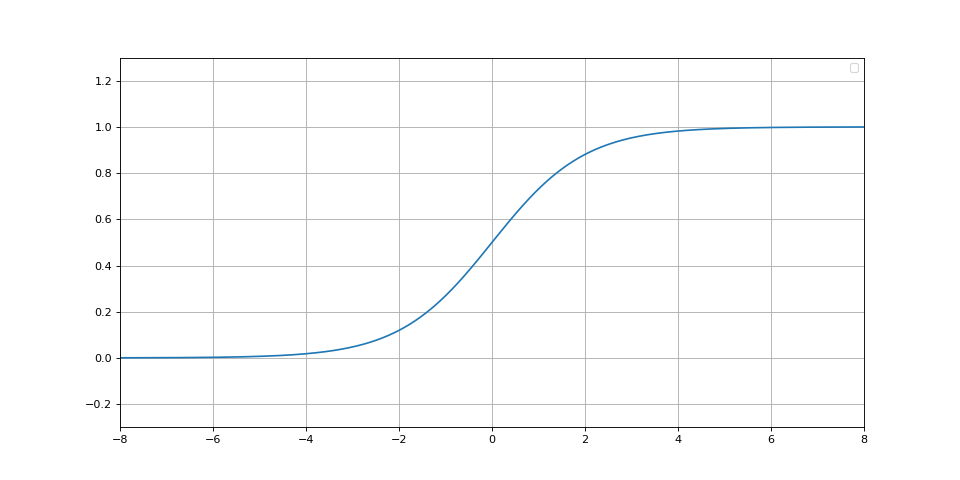
\includegraphics[width=\textwidth]{img/sigmoid.png}
      \caption{Wykres funkcji sigmoid}
      \label{sigmoid}
    \end{figure}
    
    \item funkcja softmax (liczona dla każdego neuronu warstwy wyjściowej, j = 1,...,N): 
    $$\phi(x_j) = \frac{e^{x_j}}{\sum_{k=1}^{N}{e^{x_k}}}$$
\end{itemize}

\subsubsection{Perceptron wielowarstwowy}
Jednym z pierwszych modeli Sztucznych Sieci Neuronowych był Perceptron
Wielowarstwowy (ang. MLP — \emph{Multi-Layer Perceptron}), składający 
się z warstwy neuronów wejściowej, ukrytych i wyjściowej (Rys.\ref{mlp}).
Wyjście neuronów w danej warstwie staje się wejściem neuronów warstwy następnej.

Często spotykaną wersją MLP jest model, z warstwami w pełni połączonymi
(ang. FC -- \emph{Fully Connected}). W warstwie FC każde z wyjść jest podłączone do 
wszystkich wejść neuronów w warstwie następnej.

\begin{figure}[h]
  \centering
  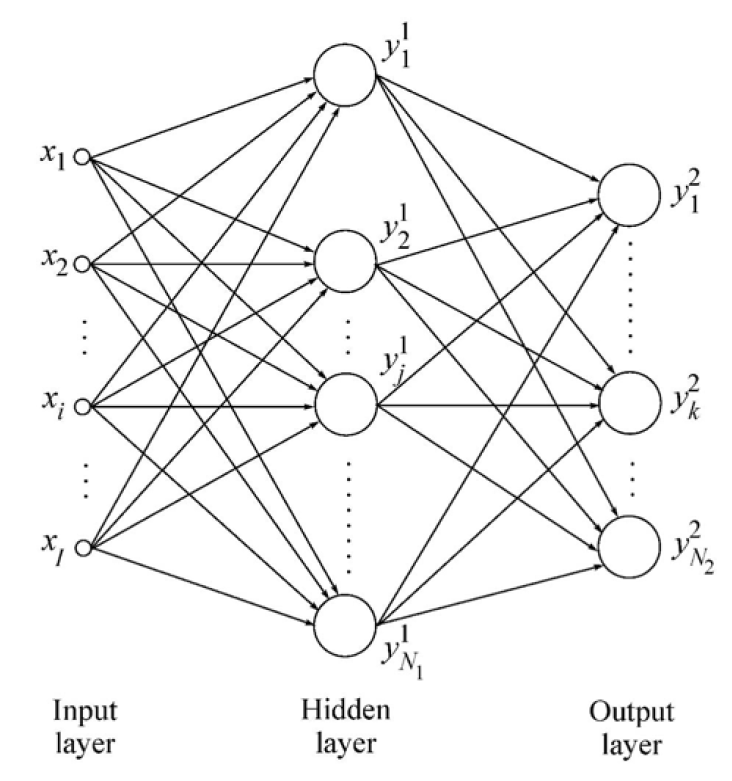
\includegraphics[width=0.9\textwidth]{img/mlp.png}
  \caption{Model Perceptronu Wielowarstwowego}
  \label{mlp}
\end{figure}


\subsubsection{Sieci Głębokie}

Rozwój algorytmów AI doprowadził do powstania Głębokich Sieci Neuronowych (ang. 
\emph{DNN — Deep Neural Networks}), czyli takich, które posiadają wiele 
warstw ukrytych\cite{Goodfellow-et-al-2016}. Algorytm Uczenia Głębokiego (ang. 
\emph{Deep Learning}) umożliwia rozwiązywanie skomplikowanych problemów takich 
jak rozpoznawanie i klasyfikację obiektów na obrazie (Rys.\ref{dnn}). Seria warstw 
ukrytych (ang. \emph{hidden layers}) umożliwia ekstrakcję cech obiektów. 
Kolejne warstwy umożliwiają wykrywanie krawędzi, potem konturów, a na końcu 
całych kształtów i obiektów.

\begin{figure}[!h]
  \centering
  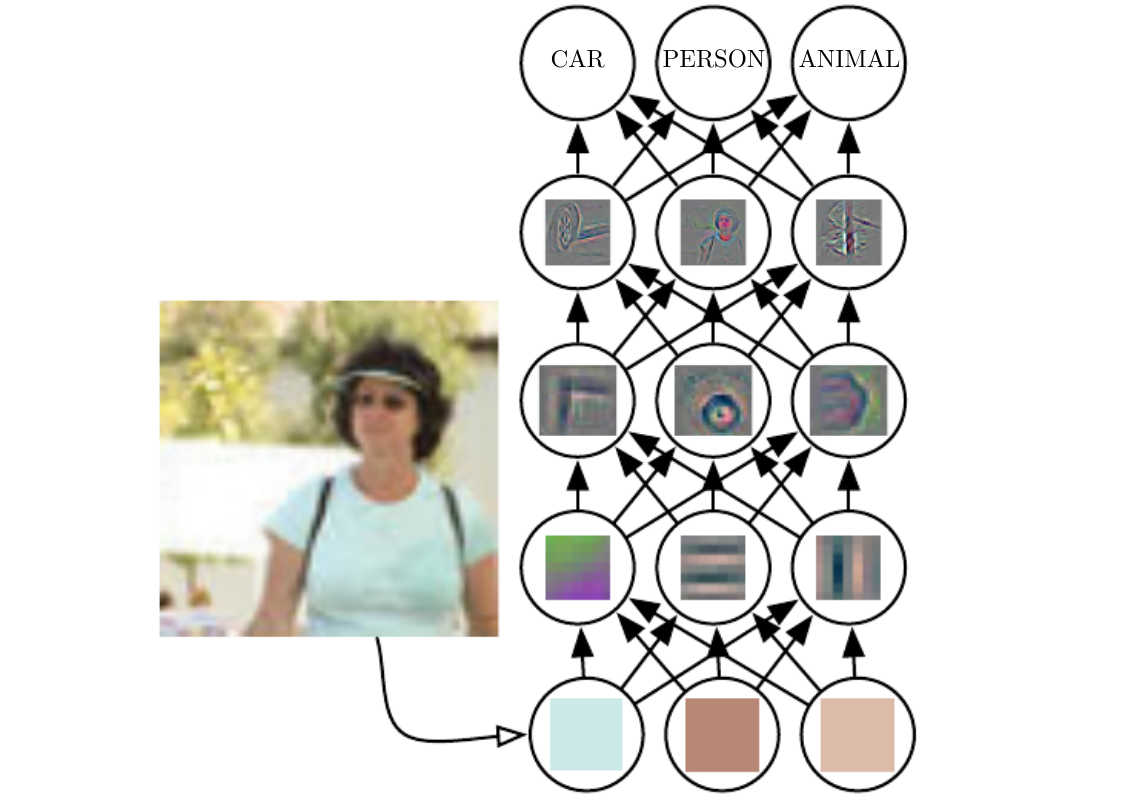
\includegraphics[width=0.8\textwidth]{img/dnn-object-recog.png}
  \caption{Model Głębokiego Uczenia sieci}
  \label{dnn}
\end{figure}


\subsubsection{Splotowe Sieci Neuronowe}

Splotowe Sieci Neuronowe (ang. \emph{CNN -- Convolutional Neural Networks}) są sieciami głębokimi, zawierającymi warstwę splotową (ang. \emph{Convolutional Layer}).
Są one z powodzeniem stosowane w wielu zagadnieniach klasyfikacji obrazów i dźwięków. 

\subsubsection{Wsteczna propagacja błędu}
Architekturę sieci MLP często stosuje się wraz z algorytmem wstecznej 
propagacji błędu (ang. \emph{Backpropagation}), która umożliwia proces uczenia sieci.
Poprzez obliczenie błędu w neuronach warstwy wyjściowej i propagacji 
wstecz błędu przez całą sieć pozwala dostosować wartość wagi każdej z krawędzi 
w taki sposób, aby zminimalizować wartość funkcji kosztu.

-learning rule (w szczególności delta rule)
-loss function
-hiperparametry
-uczenie nadzorowane/nienadzorowane


\subsection{Implementacja Sztucznych Sieci Neuronowych w układach FPGA}
\subsubsection{Reprezentacja liczb zmiennoprzecinkowych}
\subsubsection{Uczenie Sztucznej Sieci Neuronowej}
\subsection{Zastosowania Sztucznych Sieci Neuronowych}